% Szglab4
% ===========================================================================
%
\chapter{Szkeleton tervezése}

\thispagestyle{fancy}

\section{A szkeleton modell valóságos use-case-ei}
%\comment{A szkeletonnak, mint önálló programnak a működésével kapcsolatos use-case-ek.}

\subsection{Use-case diagram}

\begin{figure}[H]
\begin{center}
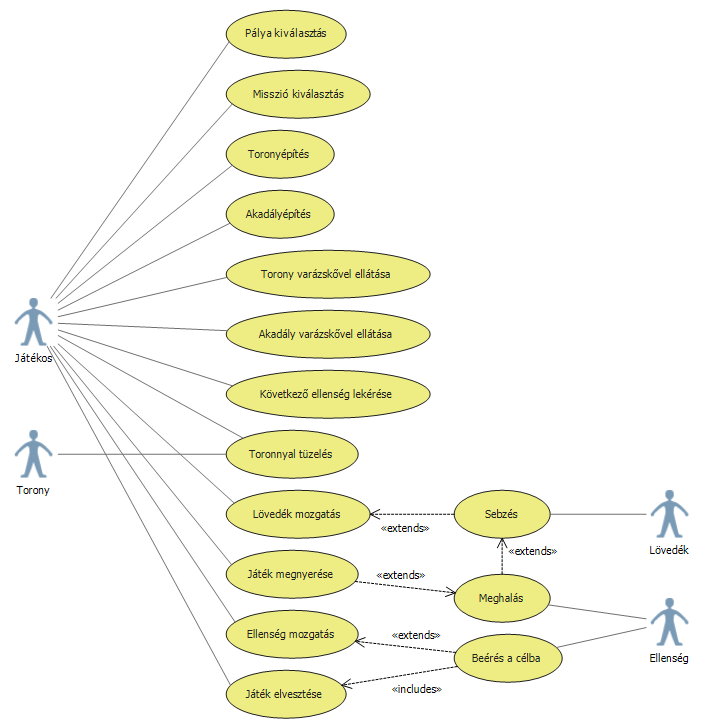
\includegraphics[width=17cm]{images/skeleton_use_case.png}
\caption{Use case diagram}
\label{fig:SzkeletonUseCase}
\end{center}
\end{figure}

\pagebreak

\subsection{Use-case leírások}
%\comment{Minden use-case-hez külön}

%Use-case neve  Rövid leírás  Aktorok  Forgatókönyv 

\usecase{Pálya kiválasztás}
{A felhasználó kiválaszt egy pályát.}
{Felhasználó}
{A program felkínál egy listát az elérhető pályák neveiről, amelyből a felhasználó kiválasztja azt, amelyiken játszani szeretne.}

\usecase{Misszió kiválasztás}
{A felhasználó kiválaszt egy missziót.}
{Felhasználó}
{A program felkínál egy listát az előzőleg kiválasztott pályán elérhető missziók neveiről, amelyből a felhasználó kiválasztja azt, amelyiken játszani szeretne.}

\usecase{Toronyépítés}
{A felhasználó felépít egy tornyot.}
{Felhasználó}
{A felhasználó megad egy pozíciót, ahova felépül egy torony.}

\usecase{Akadályépítés}
{A felhasználó felépít egy akadályt.}
{Felhasználó}
{A felhasználó megad egy pozíciót, ahova felépül egy akadály.}

\usecase{Torony varázskővel ellátása}
{A felhasználó ellát egy tornyot egy varászkővel.}
{Felhasználó}
{A felhasználó kiválaszt egy tornyot, majd egy varázskövet, amivel a toronyot erősíti.}

\usecase{Akadály varázskővel ellátása}
{A felhasználó ellát egy akadályt egy varázskővel.}
{Felhasználó}
{A felhasználó kiválaszt egy akadályt, majd egy varázskövet, amivel az akadályt erősíti.}

\usecase{Következő ellenség lekérése}
{A misszió következő ellensége elindul.}
{Felhasználó}
{A misszió soron következő ellensége létrejön, és elindul a pályán a célja felé.}

\usecase{Toronnyal tüzelés}
{Egy torony lő egyet.}
{Felhasználó, Torony}
{Egy kiválasztott torony kibocsát egy lövedéket egy megadott ellenség felé.}

\usecase{Ellenség mozgatás}
{Egy ellenség halad.}
{Ellenség}
{A kiválasztott ellenség megtesz egy lépést a célja felé vezető úton.}

\usecase{Beérés a célba}
{Egy ellenség elérte a célt.}
{Ellenség}
{Egy ellenség mozgása után elérte a célt, így a játéknak vége.}

\usecase{Játék elvesztése}
{A játék véget ér.}
{Játékos}
{A játék befejeződik, a játékos vesztett}

\usecase{Lövedék mozgatás}
{Egy lövedék halad.}
{Lövedék}
{A kiválasztott lövedék megtesz egy lépést a célpontja felé.}

\usecase{Sebzés}
{Egy lövedék célt ér.}
{Lövedék}
{Egy lövedék mozgása közben elérte a célpontját, azt megsebezte.}

\usecase{Meghalás}
{Egy ellenség életereje elfogy.}
{Ellenség}
{Ha egy lövedék célba érésekor az ellenségnek kevesebb életereje van, mint amennyit a lövedék sebez, az ellenség meghal, eltűnik.}

\usecase{Játék megnyerése}
{Az utolsó ellenség is meghal.}
{Játékos}
{Egy ellenség halálakor a játékos megnyeri a játékot, ha nincs több ellenség életben.}

\pagebreak
\setlength\parindent{15mm}
\section{A szkeleton kezelői felületének terve, dialógusok}
A szkeleton menüvezérelt módon fog működni. A felhasználónak meg kell adnia a kívánt parancsnak a kódját, majd a program lefuttatja azt. A program indítása után ki kell választani a pályát utána pedig a missziót. A menü felépítése itt látható: \\
\begingroup 
\fontsize{10pt}{10pt}\selectfont
\texttt{
1. Torony építés \\
\indent *1.1 Érvényes helyre akarunk építeni? I/N \\
\indent *1.2 Ütközik másik toronnyal? I/N \\
2. Akadály építés \\
\indent *2.1 Érvényes helyre akarunk építeni? I/N \\
\indent *2.2 Ütközik másik akadállyal? I/N \\
3. Következő ellenség lekérése \\
\indent *3.1 Van következő ellenség? I/N \\
4. Ellenség mozgatás \\
\indent *4.1 Elérte az ellenség a Waypointot? I/N \\
\indent *4.2 Hatósugarában van egy akadálynak? I/N \\
\indent \indent *4.2.1 Az akadályon van varázskő? I/N \\
5. Torony tüzelés \\
\indent *5.1 Van a tornyon varázskő? I/N \\
\indent *5.2 Van a torony hatósugarán belül ellenség? I/N \\
6. Lövedék mozgatása \\
\indent *6.1 Elérte az ellenséget? I/N \\
7. Varázskő felrakása \\
\indent *7.1 Toronyra vagy akadályra? T/A \\
\indent *7.2 Érvényes helyet adtunk meg? I/N \\
8. Ellenségek lassítása \\
\indent *8.1 Van varázskő az akadályon I/N? \\
\indent *8.2 Van ellenség az akadály hatókörében I/N? \\
9. Kilépés \\
\indent *8.1 Nyerés, vesztés, feladás vagy kilépés a programból? N/V/F/K \\
}
\endgroup \\
A *-gal jelölt menüpontokat nem lehet kiválasztani, ezt a program automatikusan megteszi, ha a felhasználó a parancs szülőjét meghívta. Ezek (1 kivétellel) igen/nem típusú kérdések. A kérdések végén láthatóak a lehetséges válaszok. A 8. pontnál  az N, V, F parancsok visszaléptetik a felhasználót a program elejére, tehát újra megkérdezi, hogy melyik pályát és missziót akarjuk kiválasztani.
\\
Az alábbi példa egy olyan interakciót mutat be, ahol a felhasználó építeni akar egy tornyot, ami érvényes helyen van, de ütközne egy másik toronnyal: \\
\begingroup
\fontsize{10pt}{10pt}\selectfont
\texttt{
? Adja meg a parancs kódját: 1 \\
- 1. Torony építése \\
>\indent ->[:Game].buildTower(pos): \\
>\indent \indent ->[:Map].canBuildTower(pos): \\
>\indent \indent \indent ->[:Waypoint].getPosition(): \\
?\indent \indent \indent 2.1. Érvényes a hely? I/N: I \\
<\indent \indent \indent <-[:Waypoint].getPosition() \\
<\indent \indent <-[:Map].canBuildTower(): \\
>\indent \indent ->[:Game].collidesWithTower(pos): \\
>\indent \indent \indent ->[:Tower].getPosition(): \\
?\indent \indent \indent 2.2. Ütközik másik toronnyal? I/N: I \\
<\indent \indent \indent <-[:Tower].getPosition() \\
>\indent \indent <-[:Game].collidesWithTower(pos) \\
>\indent <-[:Game].buildTower() \\
? Adja meg a parancs kódját:
} \\
\endgroup
\pagebreak
Minden sor elején van 1 karakter, ami a sor típusát jelöli.
\begin{itemize}
\item '?': kérdés, felhasználói interakcióra vár
\item '-': megjegyzés
\item '>': metódusba lépés
\item '<': metódusból visszatérés
\end{itemize}
A metódusba lépéskor és visszatérésnél, egy nyíl jelöli, hogy hívásról vagy visszatérésról van-e szó majd szögletes zárójelek között található az objektum típusa, ezután pedig a metódus neve. Például: ->[:Osztály].metódus():

\section{Szekvencia diagramok a belső működésre}
Az előző fejezetben lévő szekvencia diagramok továbbra is érvényesek. \\
\begin{figure}[H]
\begin{center}
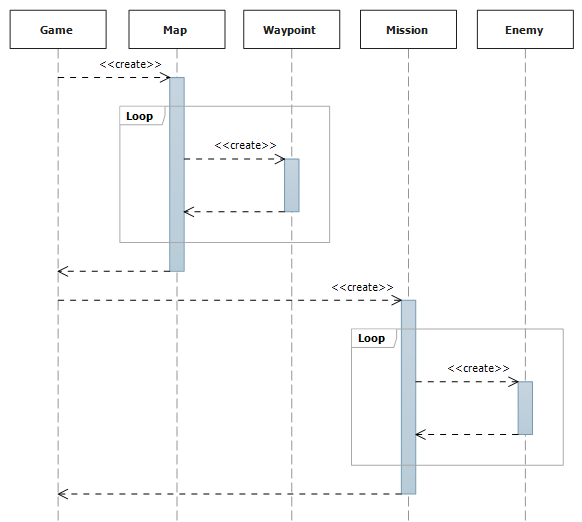
\includegraphics[width=15cm]{images/ch04/init.png}
\caption{Inicializálás. Betölti a mapet és a missiont.}
\label{fig:starting_game}
\end{center}
\end{figure}

\begin{figure}[H]
\begin{center}
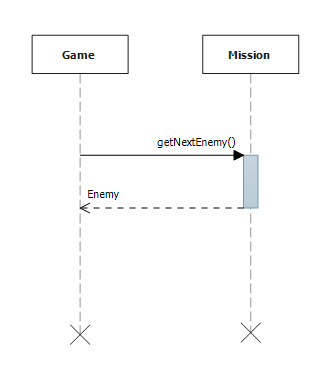
\includegraphics[width=8cm]{images/scheduling_enemies.png}
\caption{Ellenségek ütemezése.}
\label{fig:scheduling_enemies}
\end{center}
\end{figure}

\begin{figure}[H]
\begin{center}
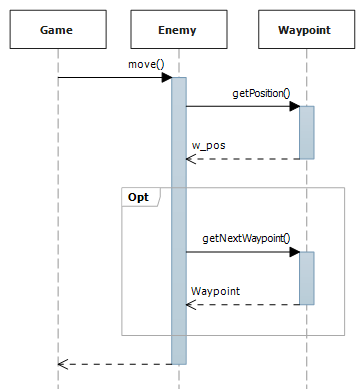
\includegraphics[width=10cm]{images/ch04/move_enemy.png}
\caption{Ellenség mozgatása. Ha elérte a waypointot lekéri a következőt.}
\label{fig:moving_enemy}
\end{center}
\end{figure}

\begin{figure}[H]
\begin{center}
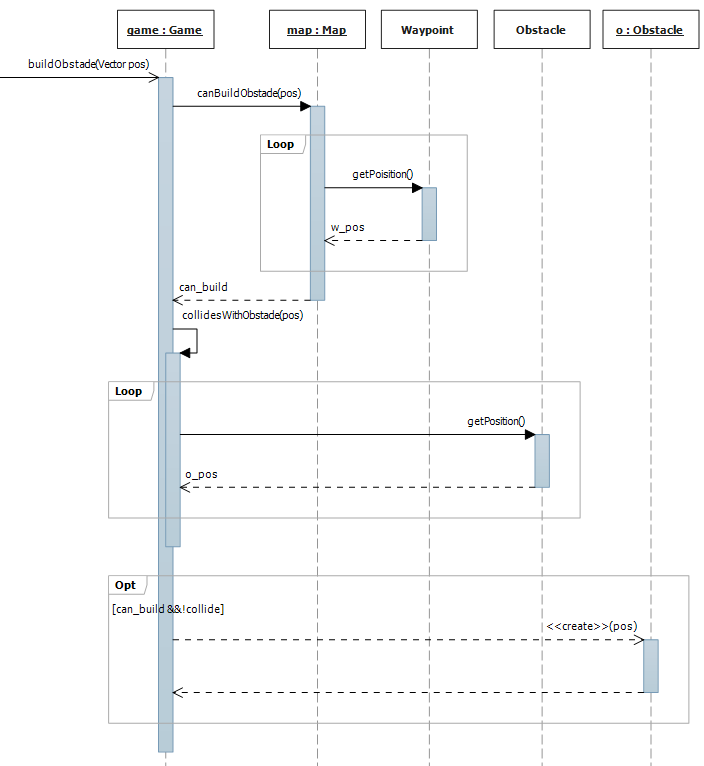
\includegraphics[width=480px]{images/ch04/build_obstacle.png}
\caption{Akadály építése. Megnézi, hogy szabad-e a helyre építeni, ha szabad épít.}
\label{fig:building_obstacle}
\end{center}
\end{figure}

\begin{figure}[H]
\begin{center}
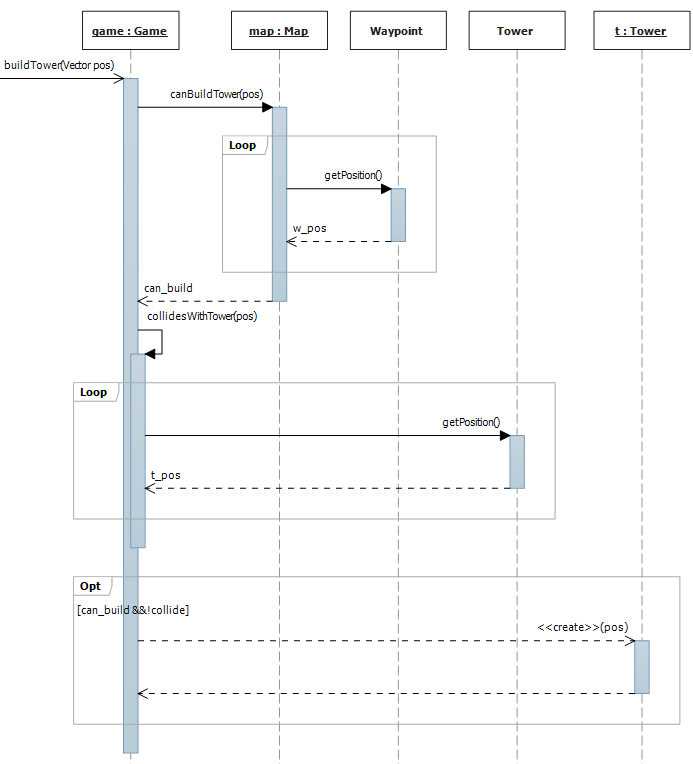
\includegraphics[width=480px]{images/ch04/build_tower.png}
\caption{Torony építése. Megnézi, hogy szabad-e a helyre építeni, ha szabad épít.}
\label{fig:building_tower}
\end{center}
\end{figure}

\begin{figure}[H]
\begin{center}
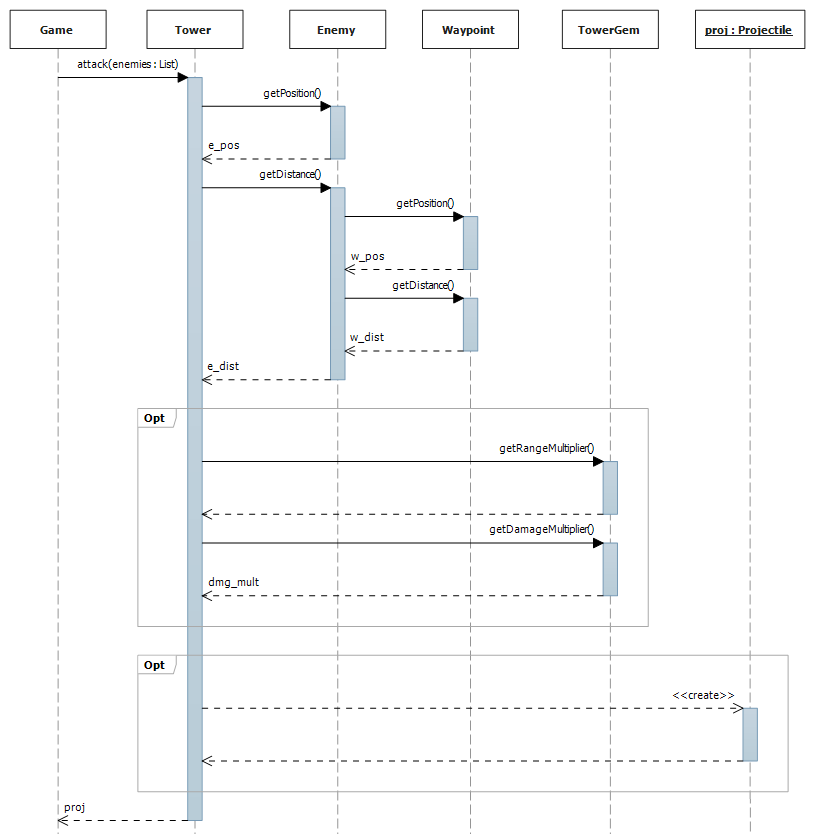
\includegraphics[width=17cm]{images/ch04/enemy_attack.png}
\caption{Ellenségek támadása. Minden ellenségre megnézi mennyire van távol a céltól és a legelsőre lő.}
\label{fig:tower_firing}
\end{center}
\end{figure}

\begin{figure}[H]
\begin{center}
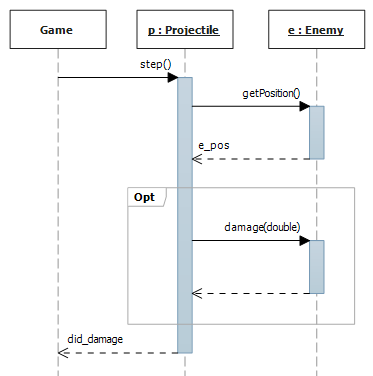
\includegraphics{images/ch04/projectile_step.png}
\caption{Lövedék léptetése.}
\label{fig:adding_gem}
\end{center}
\end{figure}

\begin{figure}[H]
\begin{center}
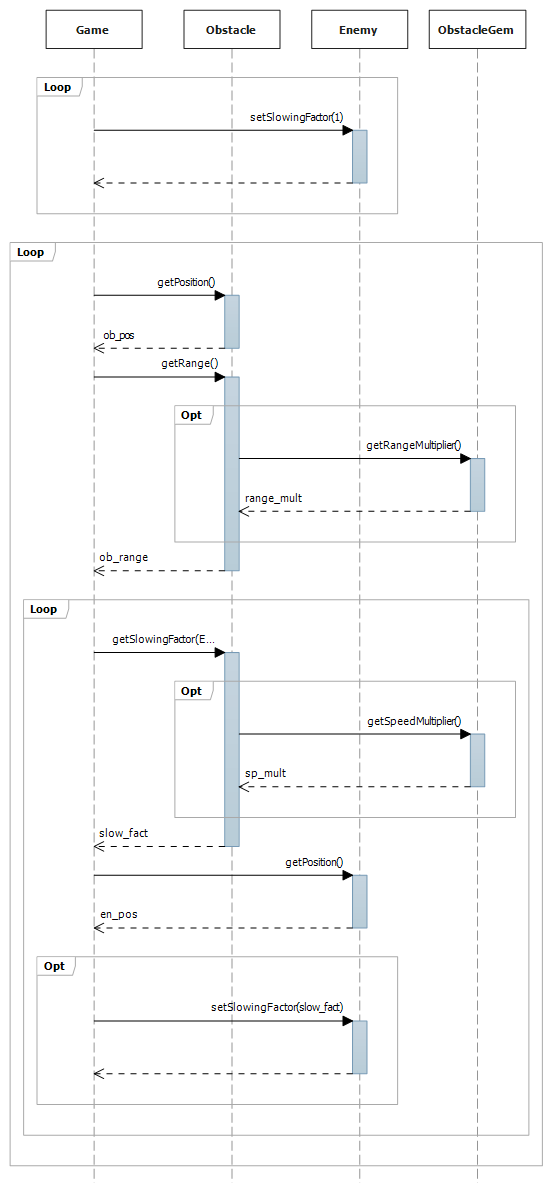
\includegraphics[width=14cm]{images/ch04/slow_enemy.png}
\caption{Minden akadály megnézi minden ellenségre, hogy a hatókörében van-e, ha igen lelassítja őket.}
\label{fig:adding_gem}
\end{center}
\end{figure}

\begin{figure}[H]
\begin{center}
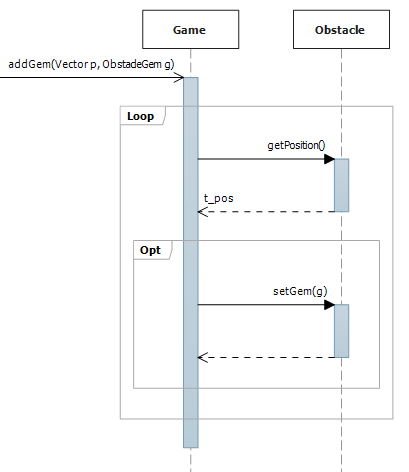
\includegraphics[width=92mm]{images/ch04/add_gem_obstacle.png}
\caption{Varázskő feltétele akadályra.}
\label{fig:adding_gem}

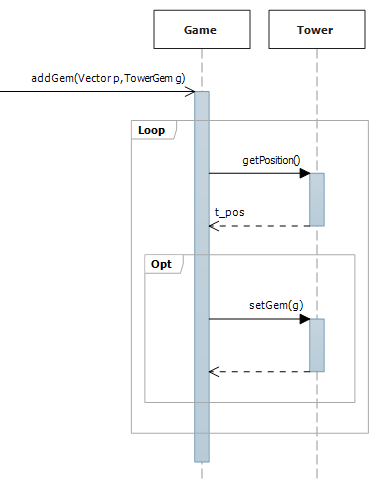
\includegraphics[width=92mm]{images/ch04/add_gem_tower.png}
\caption{Varázskő feltétele toronyra.}
\label{fig:adding_gem}
\end{center}
\end{figure}

\begin{figure}[H]
\begin{center}
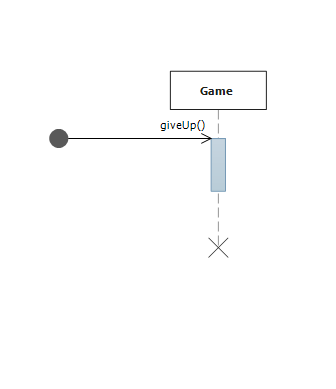
\includegraphics{images/giving_up.png}
\caption{Feladás.}
\label{fig:giving_up}
\end{center}
\end{figure}


\pagebreak

\section{Kommunikációs diagramok}
%\comment{A szkeletonban, az egyes szkeleton-use-case-ek futása során létrehozott objektumok és kapcsolataik bemutatására szolgáló %diagramok. Ezek alapján valósítják meg a szkeleton fejlesztői az inicializáló kódrészleteket.}

\begin{figure}[H]
\begin{center}
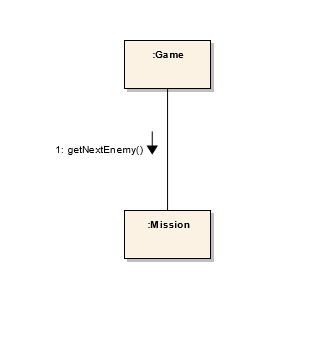
\includegraphics{images/ch05/nextEnemyKomm.png}
\caption{Ellenségek ütemezése.}
\label{fig:nextEnemyKomm}
\end{center}
\end{figure}

\begin{figure}[H]
\begin{center}
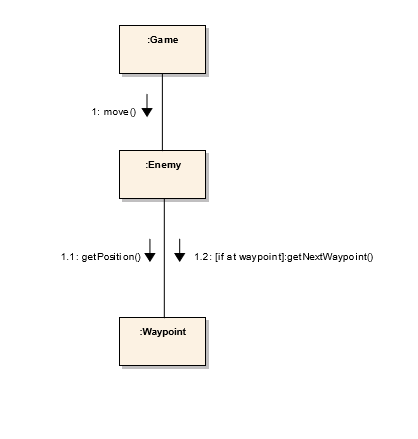
\includegraphics{images/ch05/moveKomm.png}
\caption{Ellenség mozgatása.}
\label{fig:moveKomm}
\end{center}
\end{figure}

\begin{figure}[H]
\begin{center}
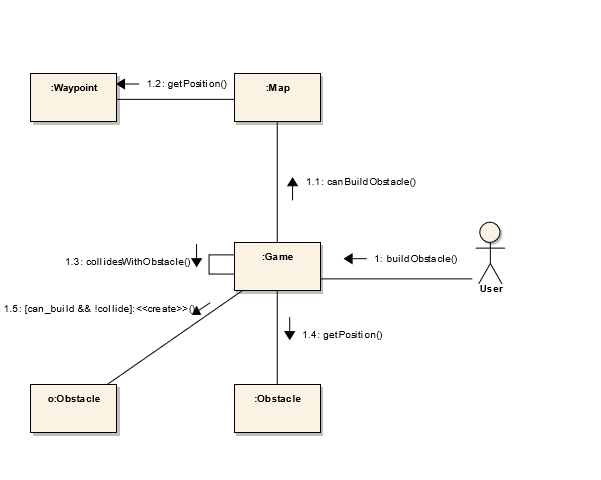
\includegraphics{images/ch05/buildObKomm.png}
\caption{Akadály építése.}
\label{fig:buildObKomm}
\end{center}
\end{figure}

\begin{figure}[H]
\begin{center}
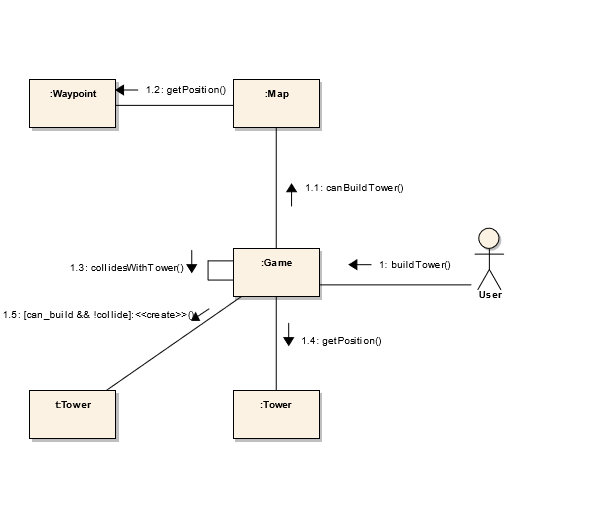
\includegraphics{images/ch05/buildTowerKomm.png}
\caption{Torony építése.}
\label{fig:buildTowerKomm}
\end{center}
\end{figure}

\begin{figure}[H]
\begin{center}
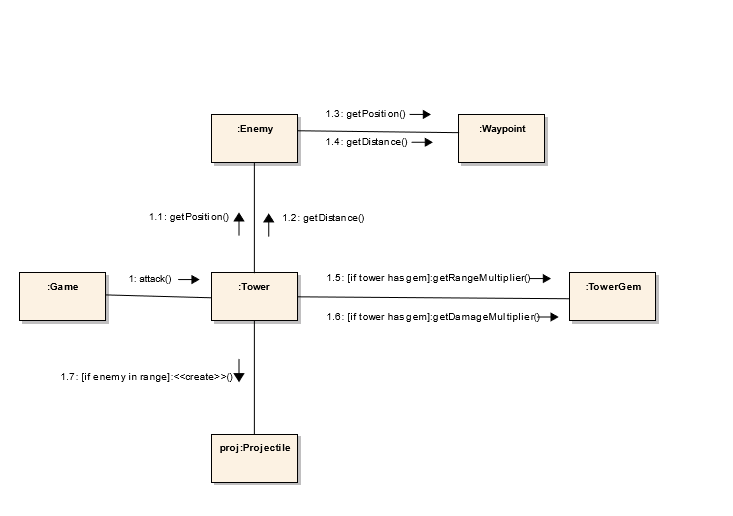
\includegraphics{images/ch05/attackKomm.png}
\caption{Torony tüzelése egy ellenségre.}
\label{fig:attackKomm}
\end{center}
\end{figure}

\begin{figure}[H]
\begin{center}
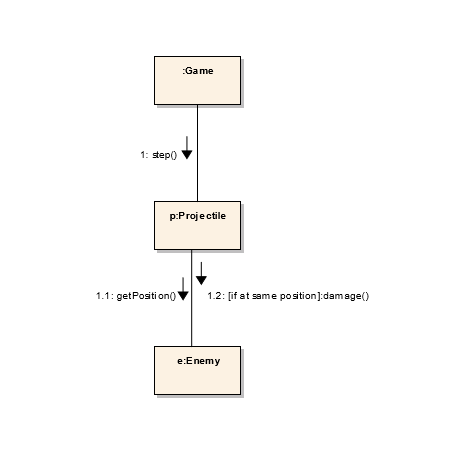
\includegraphics{images/ch05/projectileMoveKomm.png}
\caption{Lövedék mozgatása.}
\label{fig:projectileMoveKomm}
\end{center}
\end{figure}

\begin{figure}[H]
\begin{center}
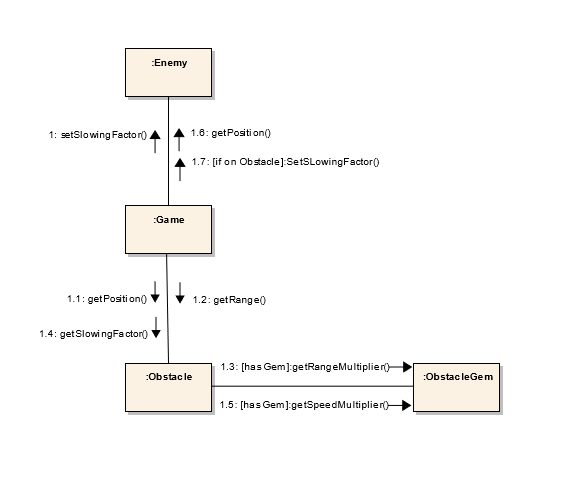
\includegraphics{images/ch05/slowKomm.png}
\caption{Akadályon áthaladó ellenség lassítása.}
\label{fig:slowKomm}
\end{center}
\end{figure}

\begin{figure}[H]
\begin{center}
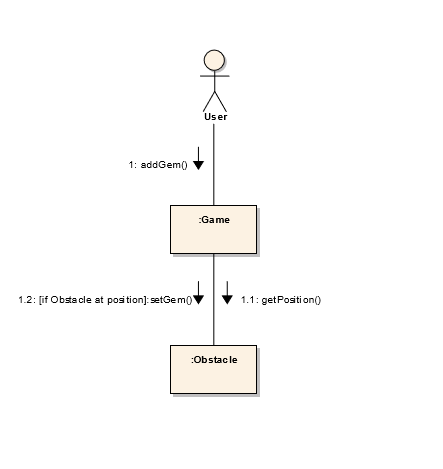
\includegraphics{images/ch05/addGemToObKomm.png}
\caption{Varázskő feltétele akadályra.}
\label{fig:addGemToObKomm}
\end{center}
\end{figure}


\begin{figure}[H]
\begin{center}
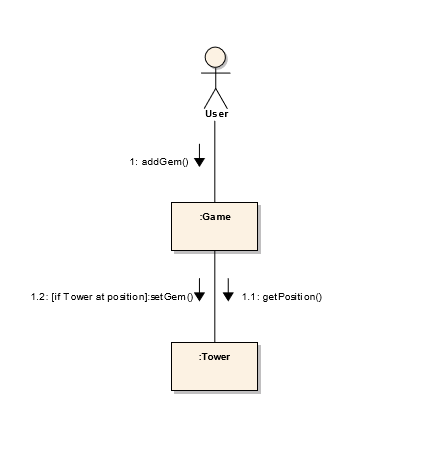
\includegraphics{images/ch05/addGemToTowerKomm.png}
\caption{Varázskő feltétele toronyra.}
\label{fig:addGemToTowerKomm}
\end{center}
\end{figure}
